%
% Listado de algoritmos implementados, análisis y diseño de generación de tokens.
% Proyecto Lovelace.
%

\section{Algoritmos tokenizadores}
\label{sec:algoritmos}

En esta sección se documentan distintos algoritmos para generar
\glspl{gl:token}; cada apartado incluye una descripción del
algoritmo y su pseudocódigo. Antes de la documentación, se presentan
dos clasificaciones de los algoritmos tokenizadores: la primera es la propuesta
por el \gls{gl:pci} \gls{gl:ssc} y mencionada en la sección \ref{sec:pci_dss}
(figura \ref{fig:division_tokens}); la segunda clasificación es propuesta por
los autores de este documento, tomando en cuenta nociones criptográficas más
estrictas (figura \ref{fig:division_propia}).

\begin{figure}[h]
  \begin{center}
    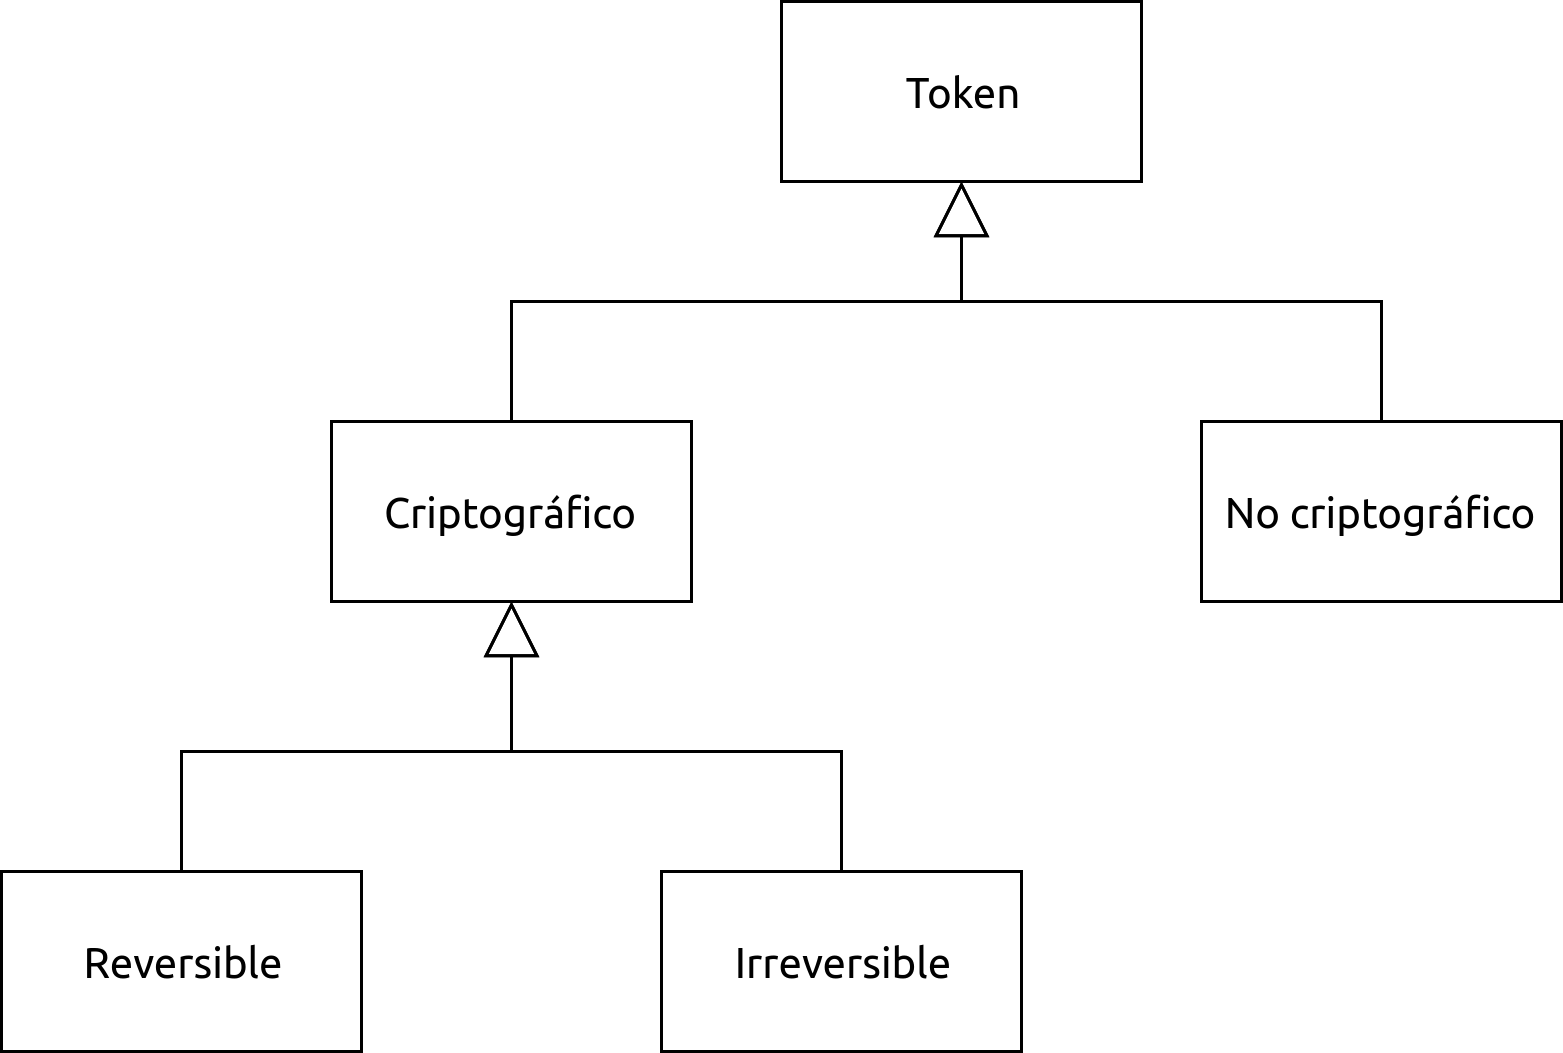
\includegraphics[width=0.75\linewidth]
      {../../../../diagramas_comunes/clasificacion/clasificacion_propia.png}
    \caption{Clasificación propia.}
    \label{fig:division_propia}
  \end{center}
\end{figure}

\paragraph{Clasificación del
  \texorpdfstring{\acrlong{gl:pci}}{PCI} \texorpdfstring{\acrlong{gl:ssc}}{SSC}}

\begin{itemize}
  \item \Glspl{gl:token} reversibles:
    \begin{itemize}
      \item \Glspl{gl:token} criptográficos:
        \begin{itemize}
          \item \Gls{gl:ffx} (véase sección~\ref{sec:ffx}).
          \item \Gls{gl:bps} (véase sección~\ref{sec:bps}).
        \end{itemize}
      \item \Glspl{gl:token} no criptográficos:
        \begin{itemize}
          \item TKR (véase sección~\ref{sec:tkr}).
          \item AHR (véase sección~\ref{sec:ahr}).
          \item \Gls{gl:drbg} (véase sección~\ref{sec:drbg_lista}).
        \end{itemize}
    \end{itemize}
\end{itemize}

Cabe resaltar que, de acuerdo con esta clasificación, los \glspl{gl:token}
generados mediante \gls{gl:drbg} pueden quedar también en la clasificación
de \gls{gl:token} no reversible, no autenticable. Se propone una nueva
clasificación, pues esta no parece muy acertada; por ejemplo, del lado de los
irreversibles se pueden generar \glspl{gl:token} autenticables (o no
autenticables) mediante funciones hash criptográficas, sin embargo, estos
\glspl{gl:token} no son \textit{criptográficos}. Respecto a los reversibles,
se toman por ejemplo, a los algoritmos TKR, que hace uso de
\glspl{gl:primitiva_criptografica}, y AHR, que hace uso de un cifrado
por bloques y una función hash criptográfica; ninguno de los cuales queda en
la categoría de los criptográficos, pues se guardan las relaciones
\gls{gl:pan}~-\gls{gl:token} en una base de datos.

\paragraph{Clasificación propuesta}

\begin{itemize}
  \item{Criptográficos}
    \begin{itemize}
      \item Reversibles:
        \begin{itemize}
          \item \Gls{gl:ffx} (véase sección~\ref{sec:ffx}).
          \item \Gls{gl:bps} (véase sección~\ref{sec:bps}).
        \end{itemize}
      \item Irreversibles:
        \begin{itemize}
          \item TKR (véase sección~\ref{sec:tkr}).
          \item AHR (véase sección~\ref{sec:ahr}).
          \item \Gls{gl:drbg} (véase sección~\ref{sec:drbg_lista}).
        \end{itemize}
    \end{itemize}
  \item No criptográficos:
    \begin{itemize}
      \item \gls{gl:nrbg}.
    \end{itemize}
\end{itemize}

La clasificación propuesta divide primeramente entre los que utilizan
criptografía y los que no; se pone como ejemplo a los item \gls{gl:nrbg} como
algoritmos no criptográficos, ya que su aleatoriedad depende de fenómenos
físicos. Luego, dentro de los criptográficos, se divide a su vez entre algoritmos
reversibles e irreversibles: los primeros, al igual que en el
\gls{gl:pci} \gls{gl:ssc}, son aquellos algoritmos que, dados el \gls{gl:token}
y la llave, pueden regresar y obtener el \gls{gl:pan}; los algoritmos
pertenecientes a la segunda subcategoría (irreversible) son aquellos que
necesitan guardar la relación \gls{gl:pan}~-\gls{gl:token} para poder obtener
el \gls{gl:pan} perteneciente a un \gls{gl:token}. Dado que, de acuerdo con el
\gls{gl:nist}, los \gls{gl:drbg} utilizan funciones hash o cifrados por
bloque, pertenecen también a la categoría de los criptográficos irreversibles.

\subimport{/}{ffx}
\subimport{/}{bps}
\subimport{/}{tkr}
\subimport{/}{rht}
\subimport{/}{drbg}
